% Draft literature review prepared for the project:
% Multi-Agent System with Temporal Fusion Transformer for Urban Air Quality Forecasting
% and Health Risk Assessment in Kazakhstan

\documentclass[pdflatex,sn-mathphys-num]{sn-jnl}

\usepackage{graphicx}%
\usepackage{multirow}%
\usepackage{amsmath,amssymb,amsfonts}%
\usepackage{mathrsfs}%
\usepackage[title]{appendix}%
\usepackage{xcolor}%
\usepackage{textcomp}%
\usepackage{manyfoot}%
\usepackage{booktabs}%
\usepackage{algorithm}%
\usepackage{algorithmicx}%
\usepackage{algpseudocode}%
\usepackage{listings}%

\raggedbottom

\begin{document}

\title[Toward an Interpretable Multi-Agent Framework for Air Quality Forecasting in Kazakhstan]{A Multi-Agent System with Temporal Fusion Transformer for Urban Air Quality Forecasting and Health Risk Assessment in Kazakhstan}

\author*[1]{\fnm{First} \sur{Author}}\email{first.author@email.com}
\author[1]{\fnm{Second} \sur{Author}}\email{second.author@email.com}

\affil*[1]{\orgdiv{Department}, \orgname{University}, \orgaddress{\city{City}, \country{Kazakhstan}}}

\abstract{Urban air pollution remains a major environmental and public health challenge in Kazakhstan, especially in cities affected by coal combustion, traffic emissions, industrial activities, and adverse meteorological conditions. Existing studies in Kazakhstan mainly focus on pollutant characterization, source apportionment, and retrospective health burden estimation, while operational forecasting and health-oriented decision support remain underdeveloped. This article presents a study design and preliminary implementation of an interpretable multi-agent system with Temporal Fusion Transformer for station-level, multi-city PM$_{2.5}$ forecasting and health risk assessment in Kazakhstan. The framework uses publicly available AirData.kz observations from Almaty, Astana, Karaganda, and other Kazakhstani locations, organizes each monitoring station as a separate time series, and maps predicted PM$_{2.5}$ concentrations into risk classes: safe, moderate, unhealthy, and hazardous. Preliminary experiments show that the best station-level multi-city TFT model achieved MAE of 11.62 $\mu$g/m$^3$ and RMSE of 17.62 $\mu$g/m$^3$ for 24-hour PM$_{2.5}$ forecasting, while the health-risk layer achieved an unhealthy-or-worse F1-score of 0.807. The study is intended to support early warning, improve interpretability in air quality forecasting, and connect environmental prediction with public-health-oriented analytics.}

\keywords{air quality forecasting, Temporal Fusion Transformer, multi-agent systems, health risk assessment, Kazakhstan, PM$_{2.5}$}

\maketitle

\section{Introduction}\label{sec:introduction}

Urban air pollution is increasingly understood as a coupled atmospheric, public health, and governance problem rather than as an isolated environmental phenomenon. Modern forecasting systems are therefore expected not only to estimate future pollutant concentrations, but also to support early warning, risk communication, and operational intervention. A broad review of air quality forecasting methods shows a clear transition from conventional statistical models toward machine learning and deep learning approaches capable of learning nonlinear interactions among pollutants, meteorological drivers, and anthropogenic variables \cite{mendez2023survey}. At the same time, public health studies continue to demonstrate that exposure to particulate matter is associated with respiratory and cardiovascular outcomes, making air quality forecasting relevant for both environmental management and health protection \cite{muratuly2025health}.

For Kazakhstan, the problem is particularly acute. Large cities such as Almaty and Astana experience heterogeneous pollution patterns shaped by coal-fired heating, combined heat and power plants, traffic emissions, industrial sources, resuspended dust, and seasonal meteorological trapping \cite{mukhtarov2023winter,ormanova2025astana,tursun2025sources}. Existing studies for Kazakhstan provide important evidence on pollutant composition, source apportionment, and economic or health burden, but comparatively little work has focused on an integrated system that is predictive, interpretable, and explicitly linked to health-oriented decision support. This gap is consequential because city authorities require not only retrospective analysis, but also actionable forecasts that help anticipate high-risk periods and prioritize protective response.

Recent advances in transformer-based time-series modeling are directly relevant in this context. Temporal Fusion Transformer (TFT) is especially promising because it supports multi-horizon forecasting, heterogeneous covariates, and interpretable feature relevance \cite{lim2021tft}. In parallel, the literature on multi-agent systems (MAS) offers mechanisms for distributed sensing, coordination, and decision routing in complex urban environments \cite{dragomir2013mas,zhu2021multisensing}. However, these two lines of research have rarely been integrated in a Kazakhstan-focused air quality application, and health risk assessment is still typically treated as a separate downstream exercise rather than as part of the operational forecasting workflow.

This article develops a near-ready methodological foundation for a study titled \textit{A Multi-Agent System with Temporal Fusion Transformer for Urban Air Quality Forecasting and Health Risk Assessment in Kazakhstan}. The current implementation focuses on hourly PM$_{2.5}$ forecasting using station-level observations from several Kazakhstani urban contexts. The paper first synthesizes the relevant literature, then identifies the research gap, formulates the research questions, proposes a reproducible methods section, and clarifies the intended scientific contribution and expected results.

\section{Literature Review}\label{sec:litreview}

\subsection{Urban air pollution and health burden in Kazakhstan}\label{subsec:kazakhstan}

The emerging literature on Kazakhstan confirms that urban air pollution is not a marginal or isolated problem. Mukhtarov et al.\ \cite{mukhtarov2023winter} analyzed wintertime PM$_{2.5}$ pollution in Almaty and showed that severe episodes are associated with persistent cold-season conditions and a combination of local emissions and atmospheric accumulation. Ormanova et al.\ \cite{ormanova2025astana} further demonstrated through chemical characterization and source apportionment that fine particulate pollution in Astana reflects multiple source categories rather than a single dominant driver. More recently, Tursun et al.\ \cite{tursun2025sources} used PMF and HYSPLIT-based analysis to show that PM$_{2.5}$ in Kazakhstan's urban centers is shaped by both local sources and air-mass transport, underscoring the need for forecasting models that can handle exogenous meteorological and trajectory-related factors.

The public-health significance of this environmental burden is also becoming more visible in the literature. Muratuly et al.\ \cite{muratuly2025health} quantified the health burden and economic costs of urban PM$_{2.5}$ pollution in Kazakhstan and argued that the magnitude of attributable mortality and welfare losses justifies stronger evidence-based management. This local evidence is consistent with global public-health guidance. The updated World Health Organization air quality guidelines emphasize that health effects occur at lower pollutant concentrations than previously assumed and identify air pollution as a major environmental health risk \cite{who2021airquality}. This line of work is important because it shifts the discussion from pollutant exceedance alone to the social consequences of exposure. However, most Kazakhstan-focused studies remain descriptive, source-oriented, or retrospective. They provide essential context for modeling, but they do not yet deliver an operational pipeline that links future pollutant levels to health-oriented alerts in a way that city authorities could use in near real time.

\subsection{From classical forecasting to machine learning and deep learning}\label{subsec:forecasting}

Air quality forecasting has historically relied on statistical methods, deterministic atmospheric models, or hybrids of the two. The broad survey by M\'{e}ndez and Casanova-Mateo \cite{mendez2023survey} shows that machine learning methods gained traction because they can learn nonlinear relations among pollutants, meteorology, land-use proxies, and anthropogenic activity indicators with fewer physical assumptions than chemistry-transport models. These data-driven methods are especially attractive when local sensor data are available but full physical simulation remains computationally expensive or operationally rigid.

Deep learning has further advanced this agenda by improving sequence modeling and multi-variate prediction. Recent operational work on automated air quality forecasting systems has shown the value of end-to-end machine learning pipelines that combine feature selection, hyperparameter optimization, and forecast generation for multiple pollutants \cite{jiao2022automated}. Multi-station forecasting research also increasingly uses spatial deep learning. Teng et al.\ \cite{teng2023gnnlstm} proposed a hybrid graph neural network for 72-hour PM$_{2.5}$ forecasting, demonstrating the importance of neighborhood spatiotemporal information for longer horizons. Mandal and Thakur \cite{mandal2023sagnn} developed a spatially attentive cluster-based graph neural network for city-level PM$_{2.5}$ forecasting, while Chen et al.\ \cite{chen2025directedgnn} used directed graph structure and meteorological fusion for regional PM$_{2.5}$ prediction. More recent graph-based work also emphasizes dynamic geographical relationships and wind-informed station interactions \cite{zhao2025dggnn}. The strength of this literature is its practical orientation toward deployment and spatial dependence. Its limitation is that many models still optimize point forecast skill without adequately addressing interpretability, transferability across cities, or direct linkage to downstream health-risk indicators.

\subsection{Transformer-based models and the relevance of Temporal Fusion Transformer}\label{subsec:tft}

Transformer architectures have become increasingly attractive for air quality forecasting because they are well suited to long-range temporal dependencies and multivariate sequence learning. Comparative reviews indicate that transformer-based models are a growing subfield within air quality prediction, particularly where long horizons, high-dimensional inputs, and multi-station data need to be handled coherently \cite{mendez2023survey}. Specific implementations support this trend. Zhang and Zhang \cite{zhang2023stn} proposed sparse attention-based transformer networks for PM$_{2.5}$ forecasting and compared them against classical machine learning and deep learning baselines. Cui et al.\ \cite{cui2023sparse} proposed a sparse attention transformer for PM$_{2.5}$ prediction and reported improvements in capturing temporal structure with reduced computational burden. Wang et al.\ \cite{wang2023msaformer} introduced MSAFormer, which combines sparse autoencoding and transformer-based prediction for multi-site meteorological features in urban PM$_{2.5}$ forecasting. Transformer-based comparisons with CNN--LSTM--attention models further suggest that self-attention can be effective for hourly PM$_{2.5}$ forecasting under changing meteorological conditions \cite{apr2023transformer}. Hu et al.\ \cite{hu2024feddeep} extended the forecasting problem to a federated multi-urban setting, indicating that distributed learning can be relevant when data ownership or infrastructure is fragmented across sites.

Within this family, TFT is especially relevant for the proposed Kazakhstan study. Lim et al.\ \cite{lim2021tft} designed TFT for interpretable multi-horizon forecasting with static covariates, known future inputs, and observed historical series. This architecture directly addresses several requirements of urban air quality forecasting: multiple exogenous drivers, changing temporal patterns, and the need to explain why the model issues a forecast. In contrast to many generic deep models, TFT offers variable selection, gating mechanisms, and attention-based interpretation. These properties are important in an applied environmental-health setting where domain experts and public agencies often require transparent reasoning rather than a purely black-box forecast.

Nevertheless, a gap remains between the promise of TFT and its application context. Most transformer-based air quality studies are developed on data from China or other high-density monitoring ecosystems, whereas Kazakhstan presents different source structure, station density, heating patterns, and policy needs. In addition, many forecasting papers evaluate model accuracy but stop short of integrating forecast outputs into a health risk layer or a coordinated monitoring-and-response framework.

\subsection{Multi-agent systems for urban air quality monitoring and decision support}\label{subsec:mas}

The literature on multi-agent systems (MAS) contributes a different but complementary perspective. Rather than focusing only on predictive accuracy, MAS research addresses distributed sensing, coordination among heterogeneous entities, and decision support. Dragomir and Oprea \cite{dragomir2013mas} presented an early multi-agent system for power-plant air pollution monitoring, showing that distributed artificial intelligence can support real-time monitoring scenarios. Zhu et al.\ \cite{zhu2021multisensing} later reviewed urban air quality monitoring and hazardous gas source analysis and proposed a conceptual framework in which mobile and static sensing agents jointly support fine-grained urban monitoring and emergency response.

These studies are useful because they conceptualize air-quality management as a coordination problem rather than as a single predictive task. However, most MAS-oriented studies emphasize sensing architecture, source search, or emergency management. They rarely incorporate state-of-the-art interpretable sequence models such as TFT, and they typically do not integrate a formal health risk assessment module. This creates a design opportunity for a new class of systems in which distributed agents manage data collection, model updating, alert generation, and decision routing while the predictive core remains transparent and multi-horizon.

\subsection{Health risk assessment as a downstream task rather than an afterthought}\label{subsec:health}

Another important strand of literature concerns the translation of pollutant concentrations into health-relevant indicators. In many urban air quality studies, health is mentioned primarily as motivation, but the analytical workflow ends at concentration forecasting. The consequence is a disconnect between environmental prediction and public-health action. Muratuly et al.\ \cite{muratuly2025health} help narrow this gap for Kazakhstan by quantifying burden and costs, while Johnson et al.\ \cite{johnson2025agent} illustrate how agent-based geospatial modeling can be used to assess PM$_{2.5}$ exposure disparities in urban airsheds. Together, these studies suggest that risk is spatially and socially heterogeneous, and that exposure-informed analytics can complement pollutant forecasting.

For the proposed project, the literature implies that forecasting alone is insufficient. A useful system for Kazakhstani cities should translate pollutant trajectories into interpretable health-oriented signals, such as exceedance warnings, exposure categories, or population-sensitive risk indices. AirNow and the U.S. Environmental Protection Agency provide an operational example of such translation through the Air Quality Index, where pollutant concentrations are mapped into color-coded health-concern categories for public communication \cite{airnow2026aqi,epa2026breakpoints}. This would align the forecasting module with the actual decision context of municipal authorities, health agencies, and vulnerable populations.

\begin{table}[h]
\caption{Summary of related work and its relevance to the proposed MAS--TFT framework.}\label{tab:related_work}
\begin{tabular}{@{}llll@{}}
\toprule
Study group & Main focus & Relevance & Remaining gap\\
\midrule
Kazakhstan PM$_{2.5}$ studies & Sources, episodes, health burden & Local scientific context & Mostly retrospective\\
Transformer forecasting & Long-range temporal dependencies & Supports TFT selection & Limited Kazakhstan evidence\\
Graph/spatial forecasting & Station interactions and transport & Supports station-level modeling & Often weak health-risk layer\\
MAS monitoring & Distributed sensing and coordination & Supports system architecture & Often lacks modern forecasting core\\
AQI and health guidance & Risk communication thresholds & Supports warning labels & Not a predictive model\\
\botrule
\end{tabular}
\end{table}

\section{Research Gap and Study Motivation}\label{sec:gap}

The literature review points to four connected gaps.

First, Kazakhstan-focused studies are expanding, but they are concentrated on pollutant characterization, source apportionment, and retrospective burden estimation rather than on integrated predictive systems \cite{mukhtarov2023winter,ormanova2025astana,tursun2025sources,muratuly2025health}. Second, advanced deep learning models for air quality forecasting are mostly developed and validated outside Central Asia, which limits confidence in their transferability to Kazakhstani cities with distinct heating, industrial, and meteorological regimes \cite{cui2023sparse,wang2023msaformer,hu2024feddeep}. Third, MAS literature provides useful concepts for distributed sensing and decision support, but it has not been tightly coupled with interpretable transformer-based forecasting \cite{dragomir2013mas,zhu2021multisensing}. Fourth, health risk assessment is usually treated as a separate downstream analysis instead of being operationally integrated into the forecasting workflow.

These gaps support a methodological and practical rationale for the proposed study. A multi-agent framework can coordinate heterogeneous data streams, local forecasting services, and alerting logic across urban locations. TFT can serve as the forecasting core because it supports multi-horizon prediction, variable heterogeneity, and interpretability. A health risk module can convert forecast pollutant concentrations into more actionable outputs for public-health communication and city management. In this sense, the proposed study is not merely another forecasting exercise; it is an attempt to bridge environmental monitoring, predictive analytics, and health-oriented decision support for Kazakhstan.

\section{Methods}\label{sec:methods}

\subsection{Study design}\label{subsec:study_design}

The proposed study is designed as a data-driven, station-level forecasting and decision-support framework for urban air quality monitoring in Kazakhstan. Instead of treating a city as a single aggregated time series, each monitoring station is represented as a separate hourly sequence. This design allows the model to learn common temporal patterns across Kazakhstan while preserving local station-specific characteristics. The initial implementation uses PM$_{2.5}$ as the target pollutant because it is both highly relevant for health risk assessment and widely represented in the available AirData.kz observations.

The study integrates three layers: a data layer, a forecasting layer, and a decision-support layer. The data layer downloads and harmonizes public hourly PM$_{2.5}$ observations for Almaty, Astana, Karaganda, and the remaining Kazakhstan station groups. The forecasting layer uses TFT as the core predictive model for 24-hour-ahead PM$_{2.5}$ prediction. The decision-support layer maps predicted pollutant concentrations into interpretable health-risk categories suitable for early warning and public-health communication.

\subsection{Data sources and variables}\label{subsec:data}

The primary dataset is AirData.kz Open Data, which provides cleaned air-quality measurements for Kazakhstan, including hourly pollutant observations grouped by city or region \cite{airdatakz2026}. The current modeling pipeline downloads hourly PM$_{2.5}$ files for Almaty, Astana, Karaganda, and the rest of Kazakhstan. Each record contains a timestamp, station identifier, station name, coordinates, source information, cluster metadata, and PM$_{2.5}$ concentration. For the multi-city model, the station identifier and city are combined into a unique series identifier, while latitude, longitude, city, and station identity are treated as static covariates.

The preprocessing pipeline converts timestamps to hourly resolution, aggregates duplicate station-hour observations by mean concentration, regularizes each station time series to an hourly grid, and interpolates only short gaps. Long missing intervals are not filled, which avoids creating artificial extended pollution episodes. The model also constructs lag and rolling-window features, including 1-hour, 24-hour, and 168-hour lags, as well as 6-hour, 24-hour, and 168-hour rolling statistics. Known future inputs include hour of day, day of week, month, day of year, weekend indicator, and heating-season indicator.

Earlier prototype models also incorporated Open-Meteo historical weather variables for Almaty, including temperature, humidity, precipitation, pressure, cloud cover, wind speed, and wind direction \cite{openmeteo2026}. These weather features improved absolute-error metrics in city-level Almaty experiments, but the current multi-city station-level baseline focuses first on PM$_{2.5}$ and calendar structure to establish a reproducible Kazakhstan-wide forecasting pipeline. Future versions should add forecast meteorology rather than only historical weather, because operational forecasting requires variables that are available before the prediction horizon.

\subsection{Multi-agent system architecture}\label{subsec:mas_arch}

The proposed MAS architecture contains several functional agents. A data acquisition agent downloads AirData.kz files and, in future operational settings, can also collect forecast meteorology. A preprocessing agent performs timestamp harmonization, duplicate aggregation, short-gap interpolation, station filtering, normalization, and feature engineering. A forecasting agent trains and executes the TFT model across multiple station-level time series. A health risk agent converts predicted PM$_{2.5}$ concentrations into categorical risk levels. A coordination agent manages experiment configuration, hyperparameter settings, and execution on local, Colab, or Kaggle environments. Finally, a reporting agent exports metrics, forecasts, checkpoints, and risk-classification outputs for further analysis.

This architecture is aligned with prior MAS literature on environmental monitoring \cite{dragomir2013mas,zhu2021multisensing}, but it extends earlier frameworks by placing an interpretable transformer model at the core of the predictive pipeline and by treating health risk estimation as a first-class system component rather than as a separate post-processing step. In implementation terms, the current system is modularized into scripts for data downloading, training, risk mapping, and evaluation, which can later be converted into independent software agents.

\begin{figure}[h]
\centering
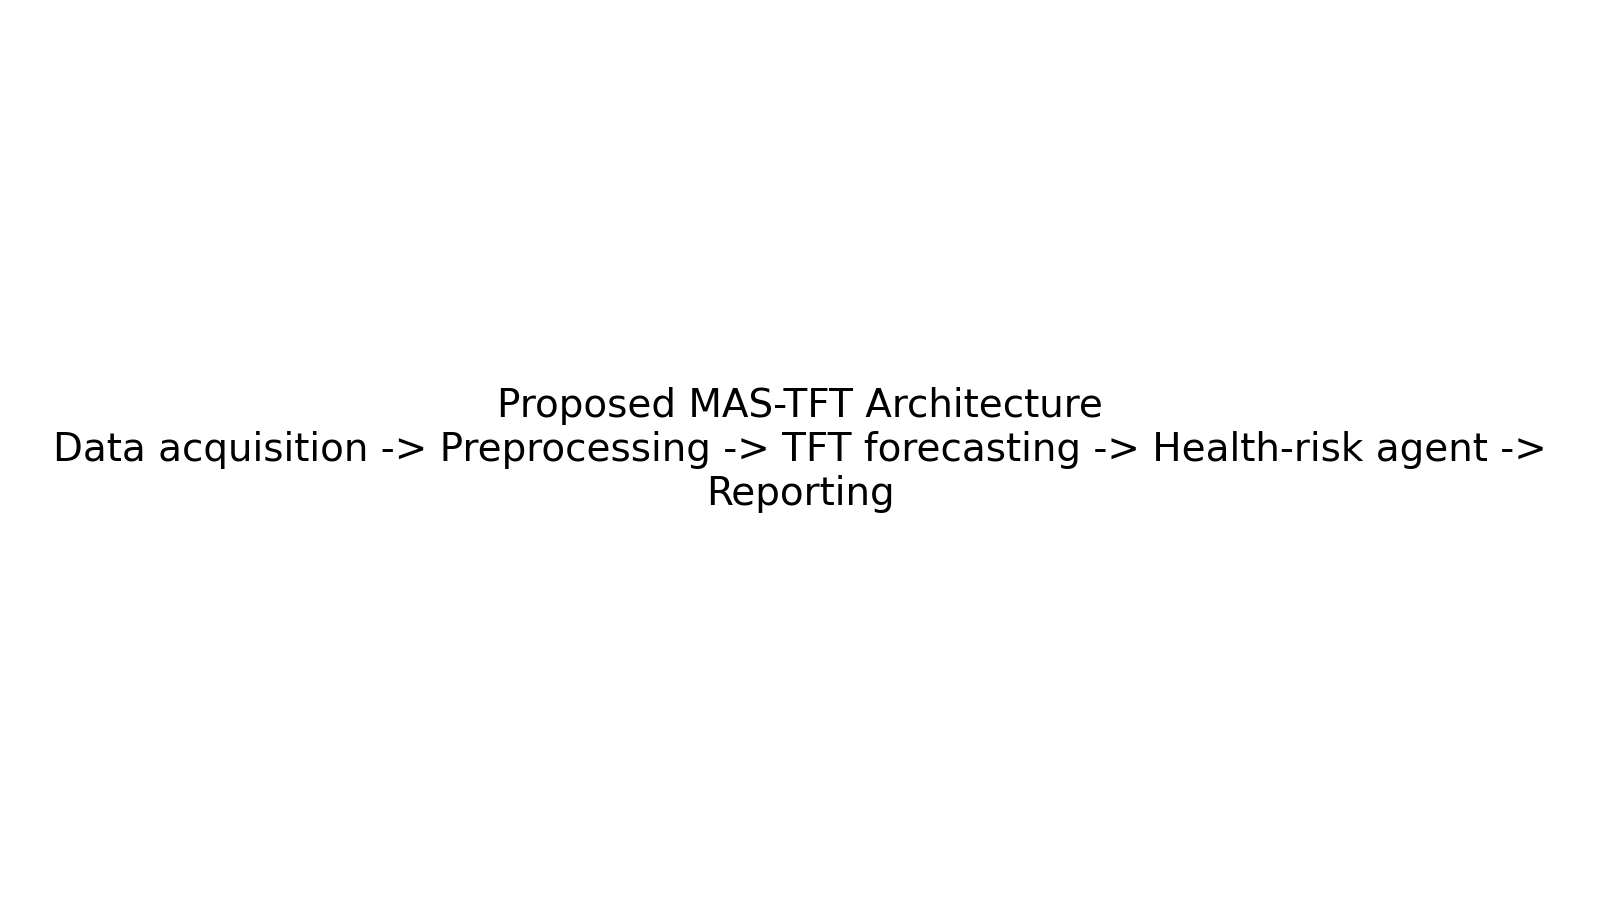
\includegraphics[width=0.85\textwidth]{figures/architecture_mas_tft.png}
\caption{Proposed multi-agent TFT framework for PM$_{2.5}$ forecasting and health-risk assessment.}
\label{fig:architecture}
\end{figure}

\subsection{Forecasting model}\label{subsec:forecasting_model}

TFT is used as the main predictive model because it can jointly handle static information, time-varying known inputs, and time-varying observed inputs while preserving interpretability through attention and variable selection mechanisms \cite{lim2021tft}. The current implementation forecasts PM$_{2.5}$ for the next 24 hours using a 168-hour encoder window. This configuration allows the model to use recent hourly dynamics as well as weekly cyclic behavior. The station-level formulation uses the combined station--city identifier as the grouping variable, so the model learns across many related time series rather than fitting one independent model per station.

The training pipeline supports hyperparameter tuning for encoder length, prediction horizon, number of stations per city, training period, hidden size, attention heads, dropout, learning rate, batch size, and maximum epochs. This is important because full multi-city station-level training is computationally heavier than a city-average model. Small smoke tests can be run on CPU, while larger experiments are intended for GPU environments such as Kaggle or Colab when available.

To evaluate whether the proposed architecture is justified, TFT should be compared with baseline models from different methodological families. These may include persistence baselines, rolling-average baselines, tree-based machine learning models such as XGBoost, recurrent networks such as LSTM, and selected transformer-based alternatives reported in the air quality literature \cite{jiao2022automated,cui2023sparse,wang2023msaformer,hu2024feddeep}. This comparative design is necessary because superior performance should be demonstrated rather than assumed.

\subsection{Health risk assessment module}\label{subsec:health_module}

The health risk module transforms both observed and predicted PM$_{2.5}$ concentrations into categorical warning labels. Separate historical health-label datasets are not required for this first stage because the labels are deterministically derived from pollutant concentrations. The current implementation uses four risk categories: safe, moderate, unhealthy, and hazardous. The thresholds are adapted from AQI-style PM$_{2.5}$ concentration breakpoints used for public risk communication \cite{airnow2026aqi,epa2026breakpoints}. In the present implementation, safe corresponds to PM$_{2.5}$ up to 12.0 $\mu$g/m$^3$, moderate to 12.1--35.4 $\mu$g/m$^3$, unhealthy to 35.5--150.4 $\mu$g/m$^3$, and hazardous to values above 150.4 $\mu$g/m$^3$. These categories are used as risk-warning proxies rather than clinical diagnoses.

The risk module compares the class derived from the actual PM$_{2.5}$ value with the class derived from the predicted PM$_{2.5}$ value. This produces classification-oriented evaluation metrics such as risk accuracy, macro F1-score, and precision, recall, and F1-score for unhealthy-or-worse events. In a health-risk early-warning system, recall for unhealthy-or-worse conditions is especially important because missed hazardous episodes are more consequential than occasional false alerts \cite{muratuly2025health,johnson2025agent}.

\subsection{Evaluation strategy}\label{subsec:evaluation}

Model performance should be evaluated with error metrics appropriate for regression forecasting, primarily MAE and RMSE. MAE is used as the most directly interpretable metric because it reports the average absolute error in $\mu$g/m$^3$. RMSE is used because it penalizes large errors more strongly and is therefore sensitive to missed pollution peaks. Percentage-based error metrics are not used as primary indicators because PM$_{2.5}$ can have very low observed values, making percentage errors unstable and potentially misleading.

Because the application includes health-risk warnings, classification-oriented metrics are also required. These include risk accuracy, macro F1-score across all risk categories, and binary precision, recall, and F1-score for unhealthy-or-worse episodes. The study should also evaluate operational value rather than accuracy alone. This means examining whether the system improves early identification of hazardous episodes, whether it preserves stable performance across stations and cities, and whether its outputs are understandable enough to support environmental and public-health decisions.

\section{Pilot Experiments and Preliminary Results}\label{sec:pilot}

Before the full multi-city station-level experiment, several pilot models were trained to validate the feasibility of the approach and to compare the effect of temporal resolution and weather covariates. These experiments used the same general TFT framework but differed in data aggregation level, input variables, and prediction setting. The pilot stage is important because it demonstrates that the pipeline can run end-to-end before scaling to a larger Kazakhstan-wide station-level model.

\begin{table}[h]
\caption{TFT experiments completed in the current project stage. Lower MAE and RMSE indicate better absolute forecasting accuracy.}\label{tab:pilot_models}
\begin{tabular}{@{}llllll@{}}
\toprule
Experiment & Scope & Main inputs & MAE & RMSE & Status\\
\midrule
Daily TFT & Almaty city-level & Daily PM$_{2.5}$ and pollutant covariates & 20.27 & 25.03 & Completed\\
Daily TFT + weather & Almaty city-level & Daily PM$_{2.5}$, pollutants, weather & 19.18 & 22.73 & Completed\\
Hourly TFT & Almaty city-level & Hourly PM$_{2.5}$, lags, rolling features & 16.60 & 20.87 & Completed\\
Hourly TFT + weather & Almaty city-level & Hourly PM$_{2.5}$, weather, temporal features & 15.02 & 19.61 & Completed\\
Multi-city station TFT & Kazakhstan station-level & Hourly PM$_{2.5}$, station metadata, temporal features & 11.62 & 17.62 & Preliminary\\
\botrule
\end{tabular}
\end{table}

The pilot results suggest three preliminary findings. First, moving from daily to hourly data improved absolute forecasting performance because the model could capture intraday variation, lagged hourly dependence, and weekly cycles. Second, adding weather variables improved MAE and RMSE in the Almaty hourly experiment. Third, the station-level multi-city formulation produced the best current MAE and RMSE among the TFT variants, suggesting that learning across multiple monitoring stations can improve the representation of urban PM$_{2.5}$ dynamics compared with a single city-level aggregate.

\begin{table}[h]
\caption{Metrics used in the forecasting and health-risk evaluation.}\label{tab:metrics}
\begin{tabular}{@{}lll@{}}
\toprule
Metric & Task & Interpretation\\
\midrule
MAE & Regression & Average absolute error in $\mu$g/m$^3$; primary accuracy metric\\
RMSE & Regression & Penalizes large errors and missed peaks more strongly than MAE\\
Risk accuracy & Classification & Share of correctly predicted risk classes\\
Macro F1 & Classification & Balanced F1-score across safe, moderate, unhealthy, hazardous classes\\
Unhealthy recall & Warning & Ability to detect unhealthy-or-worse events\\
Unhealthy F1 & Warning & Balance between false alarms and missed unhealthy events\\
\botrule
\end{tabular}
\end{table}

The full multi-city station-level model is currently in progress. This experiment uses AirData.kz hourly PM$_{2.5}$ observations from Almaty, Astana, Karaganda, and other Kazakhstani monitoring locations. Unlike the city-level pilot models, it treats each station as a separate time series and uses station identity, city, latitude, and longitude as static covariates. The experiment is designed to evaluate whether a shared TFT model can generalize across urban monitoring stations and provide both concentration forecasts and health-risk warnings. Because this run is computationally heavier, it is intended to be trained on GPU-enabled notebook environments such as Kaggle. Final multi-city results should be reported only after a complete run produces the model checkpoint, forecast file, and metrics file.

The first completed multi-city station-level evaluation used 12 station-level time series and 150,842 hourly observations. The model achieved MAE of 11.62 $\mu$g/m$^3$ and RMSE of 17.62 $\mu$g/m$^3$. For the health-risk layer, the model achieved risk accuracy of 0.674, macro F1-score of 0.440, unhealthy-or-worse precision of 1.000, unhealthy-or-worse recall of 0.676, and unhealthy-or-worse F1-score of 0.807. These preliminary results indicate that the model is conservative when issuing unhealthy-or-worse warnings: predicted unhealthy events were correct in this test window, but the model still missed approximately one third of actual unhealthy-or-worse events. Therefore, future tuning should prioritize improving unhealthy recall while preserving acceptable precision.

\begin{table}[h]
\caption{Preliminary model comparison on the shared XGBoost--TFT test overlap. Lower MAE and RMSE indicate better performance.}\label{tab:baseline_comparison}
\begin{tabular}{@{}llll@{}}
\toprule
Model & MAE & RMSE\\
\midrule
TFT & 14.42 & 20.05\\
XGBoost direct 24h & 8.05 & 11.37\\
Persistence 24h & 7.97 & 12.65\\
Rolling mean 24h & 10.77 & 14.72\\
\botrule
\end{tabular}
\end{table}

The full TFT checkpoint metrics above are computed on the complete exported TFT test set. The baseline table is computed on a smaller shared comparison subset where TFT, XGBoost, persistence, and rolling-mean predictions are all available for the same station--timestamp pairs. Therefore, the TFT value in Table~\ref{tab:baseline_comparison} differs from the full TFT metric reported in the previous paragraph. On this shared subset, the current TFT checkpoint does not yet outperform simpler baselines in MAE and RMSE. The direct 24-hour XGBoost model substantially improves over TFT in absolute-error metrics and achieves the best RMSE among the compared baselines, while persistence remains slightly better in MAE. This is a useful diagnostic result rather than a failure of the overall framework: it indicates that the current neural model is under-tuned for absolute concentration accuracy, while the risk layer already provides a meaningful warning-oriented signal. The next experimental stage should therefore include longer training, wider hyperparameter search, station-specific error analysis, weather forecast covariates, and additional machine-learning baselines before making a final performance claim.

\begin{figure}[h]
\centering
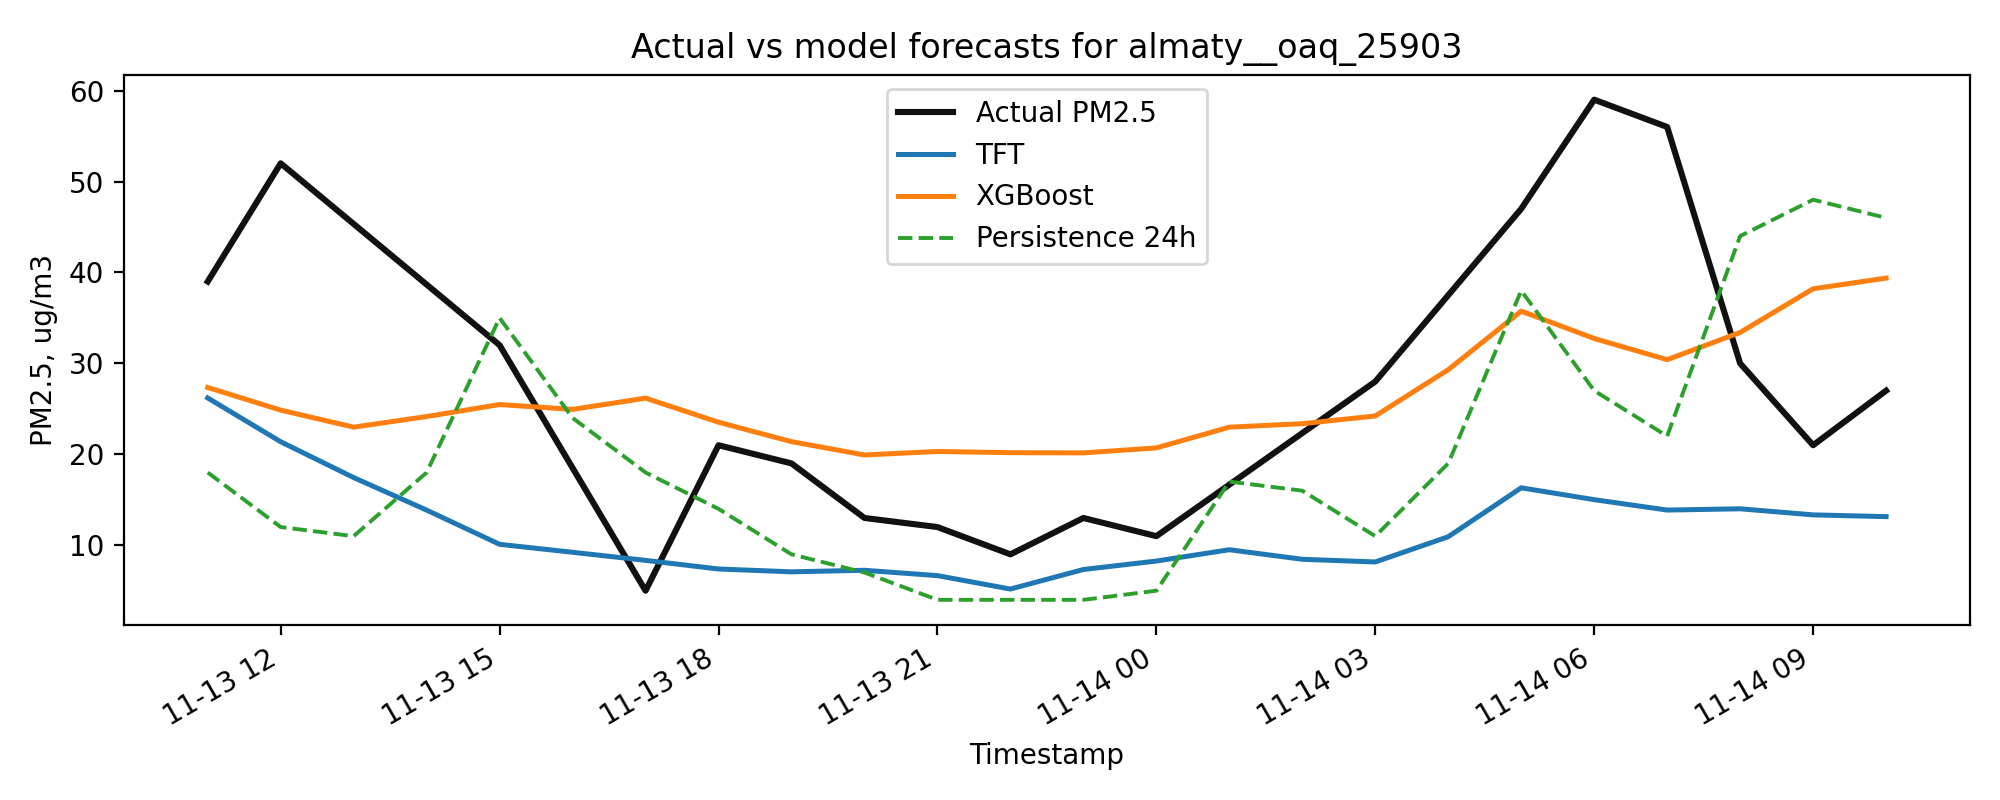
\includegraphics[width=0.85\textwidth]{figures/actual_vs_predicted_pm25.png}
\caption{Actual and predicted PM$_{2.5}$ values for a representative station-level forecast window.}
\label{fig:actual_predicted}
\end{figure}

\begin{figure}[h]
\centering
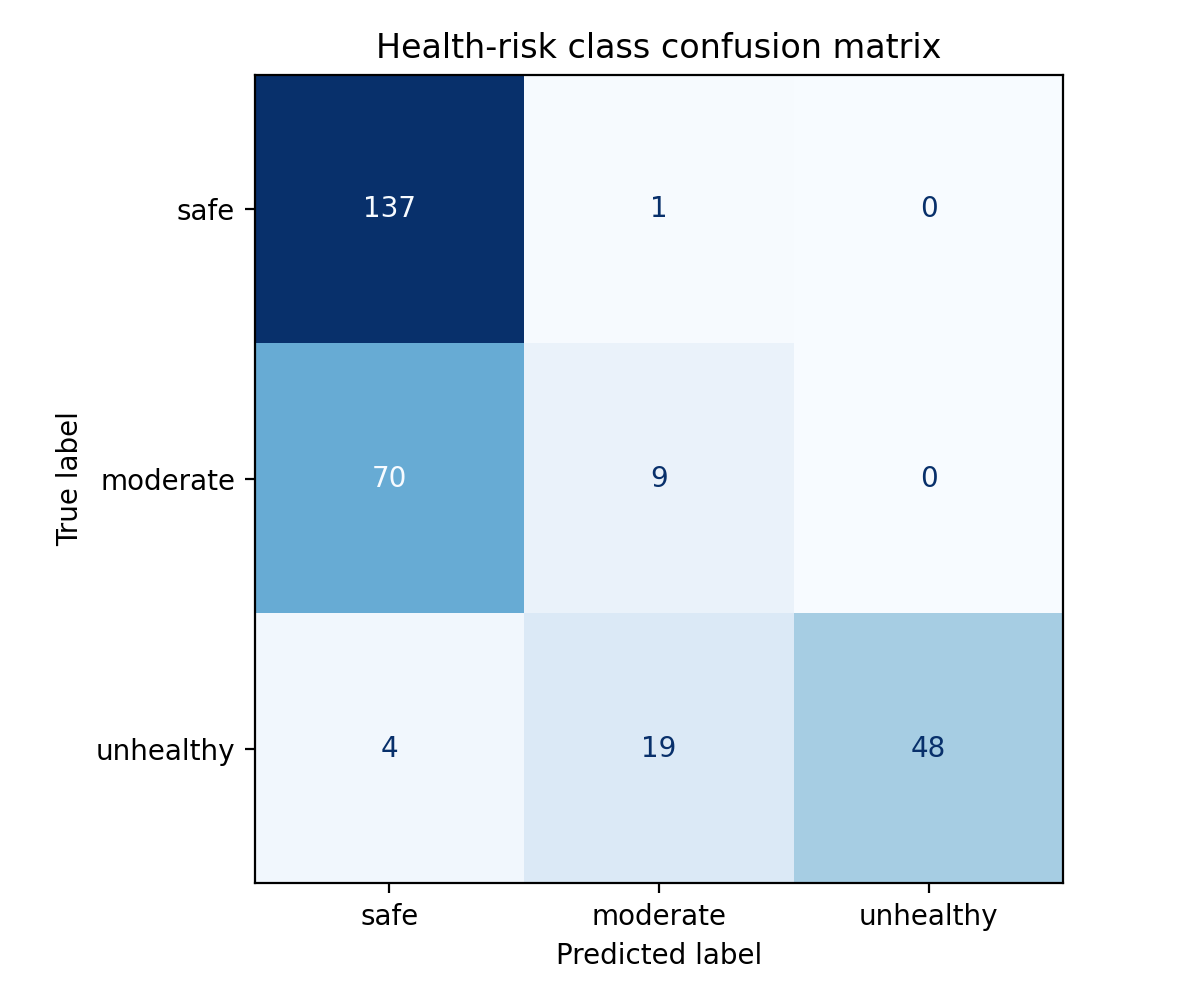
\includegraphics[width=0.72\textwidth]{figures/risk_confusion_matrix.png}
\caption{Confusion matrix for predicted and observed health-risk classes.}
\label{fig:risk_confusion}
\end{figure}

\begin{figure}[h]
\centering
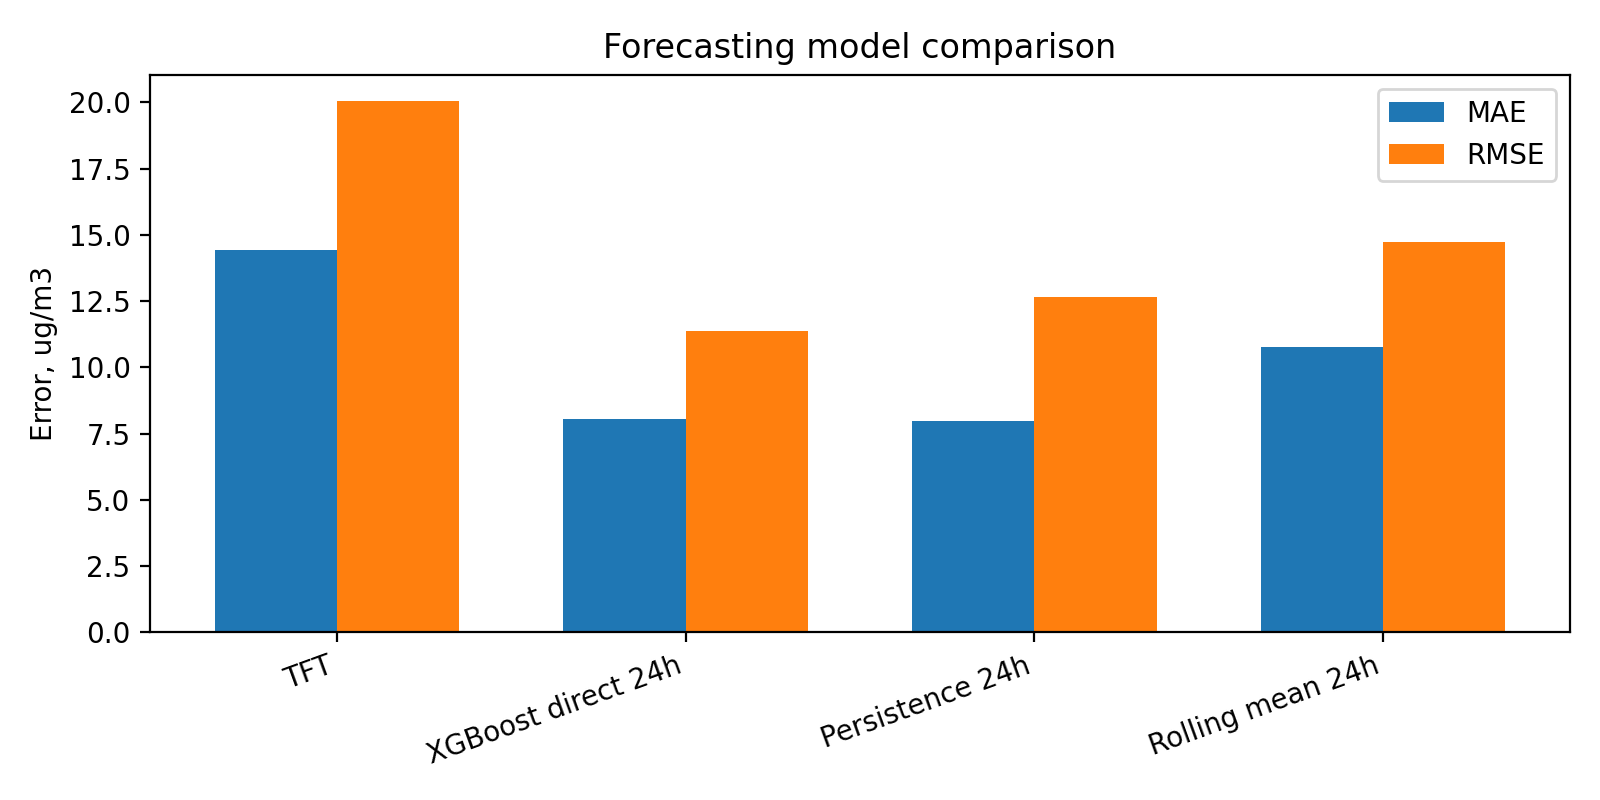
\includegraphics[width=0.78\textwidth]{figures/baseline_model_comparison.png}
\caption{Comparison between TFT, XGBoost, and simple baseline models on the imported Kaggle forecast output.}
\label{fig:baseline_comparison}
\end{figure}

\section{Discussion}\label{sec:discussion}

The preliminary experiments indicate that temporal resolution is a major factor in forecasting performance. Hourly models achieved lower MAE and RMSE than daily models because they preserve intraday pollution dynamics, short-term accumulation patterns, and lagged effects that are smoothed in daily averages. This is particularly relevant for PM$_{2.5}$, where short-lived peaks may be important for both exposure assessment and early warning.

The station-level multi-city model further improved absolute-error metrics compared with the Almaty city-level pilots. This suggests that a shared model can benefit from learning across multiple monitoring stations while still preserving local differences through station and city identifiers. The result supports the methodological choice to model each station as a separate time series rather than reducing each city to a single average concentration. However, the imported baseline comparison also shows that XGBoost and simple persistence currently outperform the TFT checkpoint in MAE and RMSE on the short test window. Therefore, the current result should be interpreted as a preliminary implementation milestone rather than a final claim of model superiority.

The evaluation focuses on MAE and RMSE rather than percentage error. This choice is important for PM$_{2.5}$ because observed concentrations can be close to zero during cleaner hours, making percentage-based metrics unstable. MAE provides a direct estimate of the average concentration error, while RMSE highlights larger misses during pollution peaks. For the public-health component, risk-oriented metrics are more appropriate for evaluating warning performance than percentage-based regression errors.

The health-risk evaluation shows a meaningful but incomplete warning capability. The preliminary multi-city model achieved unhealthy-or-worse precision of 1.000 and recall of 0.676. This means that the model was highly conservative: predicted unhealthy warnings were correct in the evaluated window, but some true unhealthy-or-worse events were missed. From a public-health perspective, future tuning should prioritize recall, because missing hazardous episodes may be more harmful than issuing some false warnings. Possible improvements include threshold calibration, longer training, more stations, weather forecast covariates, and direct optimization of warning-oriented objectives.

Several limitations remain. First, the current multi-city model uses PM$_{2.5}$ and temporal features but does not yet include forecast meteorology across all cities. Second, the current TFT checkpoint has not yet surpassed XGBoost and simple persistence in absolute-error metrics, so further tuning and additional baselines are required before drawing final conclusions. Third, the risk classes are threshold-based proxies rather than epidemiological estimates of individual health outcomes. Fourth, the computational cost of full station-level training requires GPU resources, which may limit reproducibility unless experiments are carefully documented and exported.

\section{Research Questions}\label{sec:rq}

The proposed study is guided by the following research questions:

\begin{enumerate}
\item How accurately can a station-level Temporal Fusion Transformer forecast 24-hour-ahead PM$_{2.5}$ concentrations across multiple Kazakhstani cities and monitoring stations?
\item Does a multi-city station-level formulation improve forecasting coverage and generalization compared with a single-city aggregated forecasting pipeline?
\item Which temporal and station-specific variables are most influential in TFT-based forecasts for Kazakhstani urban environments?
\item To what extent can forecast PM$_{2.5}$ concentrations be translated into interpretable health-risk categories that are useful for early warning and decision support?
\item How robust is the proposed system across cities, stations, seasons, and pollution episodes characterized by distinct source structures and atmospheric conditions?
\end{enumerate}

\section{Contribution}\label{sec:contribution}

The expected contribution of the study is threefold. First, it provides an empirical contribution by focusing on Kazakhstan, a context that is still underrepresented in advanced air quality forecasting research despite its substantial pollution burden. Second, it provides a methodological contribution by integrating MAS principles with station-level TFT-based multi-horizon forecasting in a single operational framework. Third, it provides an applied contribution by connecting PM$_{2.5}$ forecasting to a health risk assessment layer, thereby making the model outputs more actionable for decision-makers.

More specifically, the article aims to contribute an interpretable architecture that goes beyond black-box prediction, a structured workflow for combining station-level urban data streams, and a practical design for transforming environmental forecasts into public-health-relevant signals. The reproducible implementation includes scripts for downloading public Kazakhstan PM$_{2.5}$ data, training TFT models, generating PM$_{2.5}$ forecasts, deriving risk labels, and exporting results for analysis. This combination addresses empirical, methodological, and translational gaps identified in the literature review.

\section{Expected Results and Future Work}\label{sec:expected}

Several results are expected from the proposed study. First, the TFT-based approach is expected to become competitive with simple persistence, rolling-average, and machine-learning baselines after additional hyperparameter tuning, longer training, and the inclusion of forecast meteorological covariates. The current imported baseline comparison shows that this target has not yet been fully achieved for MAE and RMSE. Second, the station-level multi-city architecture is expected to improve coverage and scalability compared with a single aggregated city-level model, which is important for Kazakhstan-wide environmental analytics.

Third, the interpretability mechanisms of TFT are expected to reveal meaningful feature patterns, such as the relative importance of hourly cycles, weekly cycles, heating-season effects, station identity, and lagged pollutant dependence. These findings could provide additional scientific value beyond predictive performance alone. Fourth, the health risk module is expected to demonstrate that pollutant forecasting can be translated into clearer and more actionable decision outputs, such as exceedance warnings or risk levels for vulnerable populations.

Overall, the study is expected to show that an interpretable MAS--TFT framework can serve as a viable foundation for urban air quality early warning and health-oriented environmental analytics in Kazakhstan. Immediate future work includes improving the TFT model against naive baselines, adding tree-based baselines such as XGBoost or Random Forest, adding multi-city meteorological covariates, extending the test window, and performing interpretability analysis using TFT variable-importance and attention outputs.

\section{Conclusion}\label{sec:conclusion}

This article has transformed the initial literature review into a near-ready research paper structure for a study on a multi-agent system with TFT for urban air quality forecasting and health risk assessment in Kazakhstan. The reviewed literature indicates that Kazakhstan faces a substantial urban air pollution burden, that transformer-based forecasting methods provide promising technical capabilities, and that MAS concepts can support distributed monitoring and operational coordination. At the same time, the review highlights a clear gap at the intersection of these areas.

The proposed study addresses that gap by combining interpretable station-level forecasting, coordinated data and task management, and health-oriented decision support in a single framework. The current implementation already supports AirData.kz data downloading, multi-city station-level PM$_{2.5}$ modeling, risk-label generation, and GPU-oriented training on external notebook environments. With further refinement of experimental results, baseline comparisons, and interpretability analysis, this manuscript can serve as the foundation for a full empirical article suitable for development in Overleaf and later submission.

\backmatter

\bmhead{Acknowledgments}

This file is a project draft prepared for further refinement, journal targeting, and expansion of the reference base.

\bmhead{Data Availability}

This study uses publicly available AirData.kz Open Data for hourly PM$_{2.5}$ observations in Kazakhstan \cite{airdatakz2026}. Prototype weather-enhanced experiments use Open-Meteo historical weather data \cite{openmeteo2026}. Processed datasets and model outputs are generated by the project scripts and can be reproduced from the public data sources.

\bibliography{kz-air-quality-review-bib}

\end{document}
